\documentclass[11pt, a4paper]{article}
\usepackage[utf8]{inputenc}
\usepackage[T1]{fontenc}
\usepackage[norsk]{babel}
\usepackage{hyperref}
\usepackage{fancyvrb}
\usepackage{marginnote}

\usepackage{tgheros}
\renewcommand*\familydefault{\sfdefault}

\usepackage{xspace}
\newcommand{\TikZ}{Ti\textit{k}Z\xspace}

\newcommand\Oppgave{\reversemarginpar\marginnote {\textcolor{orange}{Utfordring}}}

\usepackage{tikz}
\usepackage{circuitikz}

\usepackage{amsmath}

\usetikzlibrary{automata}
\usetikzlibrary{shapes}
\usetikzlibrary{mindmap}
\usetikzlibrary{calendar}

\title{Tegnekurs i \TikZ}
\author{Veronika Heimsbakk \\ veronahe@ifi.uio.no}

\begin{document}

\maketitle
\tableofcontents
\listoffigures


\section*{Introduksjon}
Dette er et «kompendie», eller et sammendrag av «Tegnekurs i TeX» arrangert av studentforeningen \{ProgNett\} 6. oktober 2014 ved Institutt for informatikk, Universitetet i Oslo.

Dokumentet du nå leser er lagt opp slik at du skal kjenne til \TeX/\LaTeX fra før, men ikke nødvendigvis pakken \TikZ. Per dags dato, \today, så fins ingen engelsk versjon av dette dokumentet. Men det er underveis.

Hvis du har spørsmål, finner feil, eller har andre tilbakemeldinger. Send dette til forfatteren Veronika Heimsbakk, \href{mailto:veronahe@ifi.uio.no}{veronahe@ifi.uio.no}.

\newpage

%%% BASICS %%%
\section{The Basics}
For å kunne bruke pakken \TikZ må man først inkludere pakken i dokumentet.
\begin{Verbatim}[fontsize=\small]
\usepackage{tikz}
\end{Verbatim}

\subsection{\texttt{tikzpicture}}
Alle illustrasjoner som skal tegnes ved hjelp av pakken \TikZ krever et miljø som heter \texttt{tikzpicture}.

\begin{Verbatim}[fontsize=\small]
\begin{tikzpicture}
    <kode her>
\end{tikzpicture}
\end{Verbatim}

% Linjer
\subsection{Linjer}
\begin{center}
\begin{tikzpicture}
	\draw (0,2) -- (4,2);
	\draw (0cm,1.5cm) -- (4cm,1.5cm);
	\draw (0em, 1cm) -- (4em, 1cm);
	\draw (0pt, 0.5cm) -- (4pt, 0.5cm);
\end{tikzpicture}
\end{center}

En av de mest brukte \TikZ kommandoene er \texttt{\textbackslash draw}. For å tegne ei rett linje sier man hvor man vil tegne \textit{fra} og \textit{til}:

\begin{Verbatim}[fontsize=\small, frame=single]
\draw (0,2) -- (4,2);
\draw (0cm,1.5cm) -- (4cm,1.5cm);
\draw (0em, 1cm) -- (4em, 1cm);
\draw (0pt, 0.5cm) -- (4pt, 0.5cm);
\end{Verbatim}
Koordinatene \texttt{(0,2)} sier at vi skal starte linjen i $x=0$ og $y=2$.

% Kurver
\subsection{Kurver}
Vi bruker kontrollpunkter for å lage en kurvet linje. I eksempelet her, så starter vi i koordinatene \texttt{(-2,2)} og så tegner vi en kurve til første kontrollpunkt som er \texttt{(-1,0)}, så videre til \texttt{(1,0)}, og til slutt ender kurven opp i slutt-punktet som er \texttt{(2,2)}.

\begin{center}
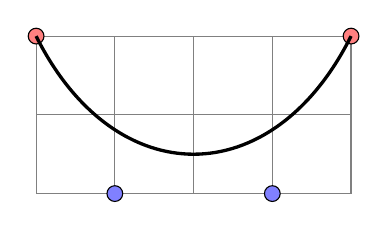
\begin{tikzpicture}
	\draw[black!50] (-2,0) grid (2,2);
	\draw[fill=red!50] (-2,2) circle (0.1cm);
	\draw[fill=blue!50] (-1,0) circle (0.1cm);
	\draw[fill=blue!50] (1,0) circle (0.1cm);
	\draw[fill=red!50] (2,2) circle (0.1cm);
	\draw[black, very thick] (-2,2) .. controls (-1,0) and (1,0) .. (2,2);
\end{tikzpicture}
\end{center}

\begin{Verbatim}[fontsize=\small]
\draw (-2,2) .. controls (-1,0) and (1,0) .. (2,2);
\end{Verbatim}

\newpage

% Kvadrat
\subsection{Kvadrat}
Vi kan bygge på linjen vår og lage et kvadrat:
\begin{center}
\begin{tikzpicture}
	\draw (0,0) rectangle (1.5,1.5);
\end{tikzpicture}
\end{center}

\begin{Verbatim}[fontsize=\small]
\draw (0,0) -- (1.5,0) -- (1.5,1,5) -- (0,1.5) -- (0,0);
\end{Verbatim}
Vi kan også bruke nøkkelordet \texttt{rectangle}, og lage en kortversjon som gjør akkurat det samme:
\begin{Verbatim}[fontsize=\small]
\draw (0,0) rectangle (1.5,1.5);
\end{Verbatim}

% Sirkler
\subsection{Sirkel}
\begin{center}
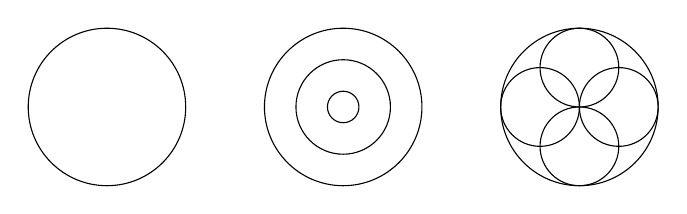
\begin{tikzpicture}
	\draw (0,0) circle (1cm);
	\draw(3,0) circle (1cm) circle (0.6cm) circle (0.2cm);
	\draw(6,0) circle (1cm);
	\draw(6.5,0) circle (0.5cm);
	\draw (6,0.5) circle (0.5cm);
	\draw(5.5,0) circle (0.5cm);
	\draw(6,-0.5) circle (0.5cm);
\end{tikzpicture}
\end{center}

Den første koordinaten er sirkelens sentrum, og lengden vi oppgir til slutt er sirkelens radius. 

\begin{Verbatim}[fontsize=\small]
\draw (0,0) circle (1cm);
\end{Verbatim}
\Oppgave
Hvordan tegnes figurene 
\scalebox{0.2}{
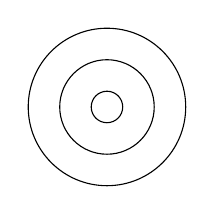
\begin{tikzpicture}
	\draw(3,0) circle (1cm) circle (0.6cm) circle (0.2cm);
\end{tikzpicture}
} 
og
\scalebox{0.2}{
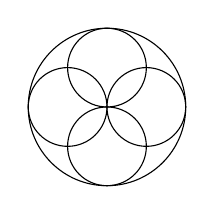
\begin{tikzpicture}
	\draw(6,0) circle (1cm);
	\draw(6.5,0) circle (0.5cm);
	\draw (6,0.5) circle (0.5cm);
	\draw(5.5,0) circle (0.5cm);
	\draw(6,-0.5) circle (0.5cm);
\end{tikzpicture}
} 
?

% Ellipser
\subsection{Ellipse}
\noindent Ellipser tegnes ved at vi oppgir radiusen i x- og y-retningene:
\begin{center}
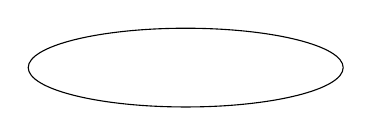
\begin{tikzpicture}
	\draw (0,0) ellipse (2cm and 0.5cm);
\end{tikzpicture}
\end{center}

\begin{Verbatim}[fontsize=\small]
\draw (0,0) ellipse (2cm and 0.5cm);
\end{Verbatim}

% Arc
\subsection{Buer}
\begin{center}
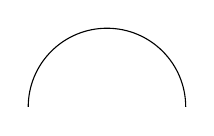
\begin{tikzpicture}
	\draw (0,0) arc (0:180:1);
\end{tikzpicture}
\end{center}

\noindent Buer (\texttt{arc}) skriver man på formen

\begin{Verbatim}[fontsize=\small]
\draw  (0,0) arc (0:180:1);
\end{Verbatim}
Hvor \texttt{(0,0)} er posisjonen. Og \texttt{(0:180:1)} betyr at vi skal tegne en bue fra 0 til 180 grader på en sirkel med radius 1.

\newpage 

% Pynte på sirkler
\subsection{Pynte litt}
For å pynte litt på sirkelen vår, kan vi legge til noen ekstra argumenter på \texttt{\textbackslash draw}-kommandoen. For eksempel slik:
\begin{center}

\begin{tikzpicture}
	\draw[red, thick, dashed] (2,2) circle (1cm);
	\draw[green, thick] (6,2) circle (1cm);
\end{tikzpicture}
\end{center}

\begin{Verbatim}[fontsize=\small]
\draw[red, thick, dashed] (2,2) circle (1cm);
\draw[green, thick] (6,2) circle (1cm);
\end{Verbatim}

% Tykkelser
\subsection{Tykkelser}
\begin{minipage}{0.4\textwidth}
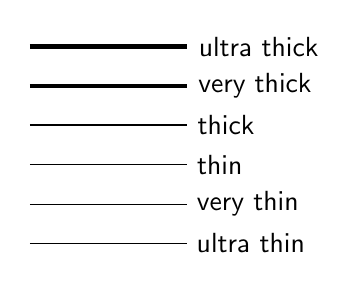
\begin{tikzpicture}
	\draw[ultra thin] (0,0) -- (2,0) node[right] {ultra thin};
	\draw[very thin] (0,0.5) -- (2,0.5) node[right] {very thin};
	\draw[thin] (0,1) -- (2,1) node[right] {thin};
	\draw[thick] (0,1.5) -- (2,1.5) node[right] {thick};
	\draw[very thick] (0,2) -- (2,2) node[right] {very thick};'
	\draw[ultra thick] (0,2.5) -- (2,2.5) node[right] {ultra thick};
\end{tikzpicture}
\end{minipage}
\begin{minipage}{0.5\textwidth}
\noindent Man kan også definere egne tykkelser ved å bruke \texttt{line width}.
\begin{center}

\begin{tikzpicture}
	\draw[line width=10pt] (0,0) -- (2,0);
\end{tikzpicture}
\end{center}
\begin{Verbatim}[fontsize=\small]
\draw[line width=10pt] (0,0) -- (2,0);
\end{Verbatim}
\end{minipage}



% Farger
\subsection{Farger}
\begin{figure}[h!]
\centering
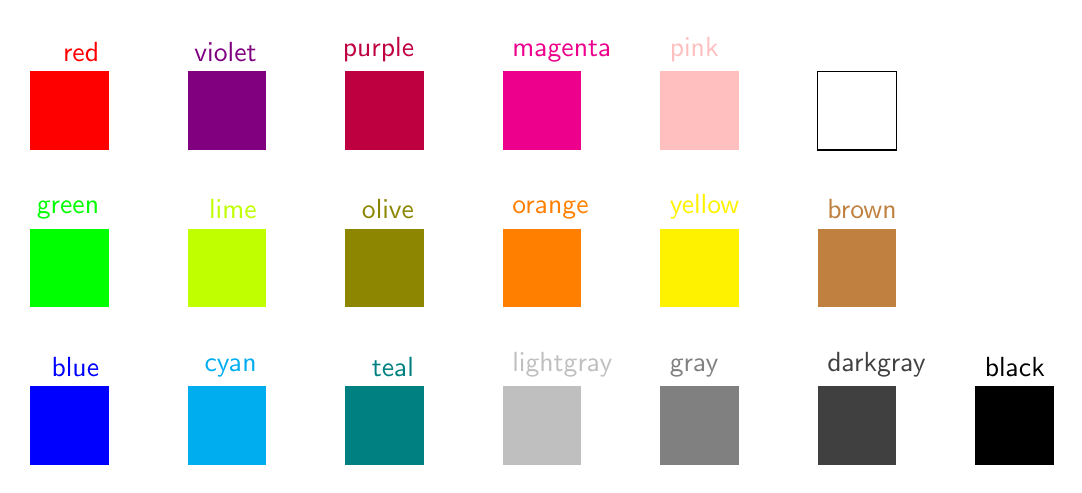
\begin{tikzpicture}
	\fill[red] (0,4) rectangle (1,5) node[above left] {red};
	\fill[violet] (2,4) rectangle (3,5) node[above left] {violet};
	\fill[purple] (4,4) rectangle (5,5) node[above left] {purple};
	\fill[magenta] (7,4) rectangle (6,5) node[above right] {magenta};
	\fill[pink] (9,4) rectangle (8,5) node[above right] {pink};
	\fill[white, draw=black, thin] (11,4) rectangle (10,5) node[above right] {white};

	\fill[green] (0,2) rectangle (1,3) node[above left] {green};
	\fill[lime] (2,2) rectangle (3,3) node[above left] {lime};
	\fill[olive] (4,2) rectangle (5,3) node[above left] {olive};
	\fill[orange] (7,2) rectangle (6,3) node[above right] {orange};
	\fill[yellow] (9,2) rectangle (8,3) node[above right] {yellow};
	\fill[brown] (11,2) rectangle (10,3) node[above right] {brown};

	\fill[blue] (0,0) rectangle (1,1) node[above left] {blue};
	\fill[cyan] (2,0) rectangle (3,1) node[above left] {cyan};
	\fill[teal] (4,0) rectangle (5,1) node[above left] {teal};
	\fill[lightgray] (7,0) rectangle (6,1) node[above right] {lightgray};
	\fill[gray] (9,0) rectangle (8,1) node[above right] {gray};
	\fill[darkgray] (11,0) rectangle (10,1) node[above right] {darkgray};
	\fill[black] (13,0) rectangle (12,1) node[above right] {black};
\end{tikzpicture}
\caption{Farger i \TikZ.}
\end{figure}

\newpage

% Bruke farger
\subsection{Fylle med farge}
Vi kan også fylle formene våre med farger ved å bruke kommandoen \texttt{\textbackslash fill}.
Ønsker vi å legge til en kant rundt kvadratet, kan vi bruke kommandoen \texttt{\textbackslash filldraw}.

\begin{center}

\begin{tikzpicture}
	\fill[orange] (0,0) rectangle (2,2);
	\filldraw[orange, draw=black, very thick] (3,0) rectangle (5,2);
\end{tikzpicture}
\end{center}

\begin{Verbatim}[fontsize=\small]
\fill[orange] (0,0) rectangle (2,2);
\filldraw[orange, draw=black, very thick] (3,0) rectangle (5,2);
\end{Verbatim}

% Gradient
\subsubsection{Gradient}
\noindent Vi har også gradient i \TikZ, og det kan se slik ut:

\begin{center}

\begin{tikzpicture}
	\shade[left color=orange, right color=yellow] (0,0) rectangle (2,2);
	\shade[top color=orange, bottom color=yellow] (3,0) rectangle (5,2);
	\shade[inner color=orange, outer color=yellow] (6,0) rectangle (8,2);
\end{tikzpicture}
\end{center}

\begin{Verbatim}[fontsize=\small]
\shade[left color=orange, right color=yellow]  (0,0) rectangle (2,2);
\shade[top color=orange, bottom color=yellow]  (3,0) rectangle (5,2);
\shade[inner color=orange, outer color=yellow] (6,0) rectangle (8,2);
\end{Verbatim}
\Oppgave
Hvordan tegner vi dette
\scalebox{0.2}{

\begin{tikzpicture}
	\shade[inner color=orange, outer color=white] (6,0) rectangle (8,2);
\end{tikzpicture}
}
?

% Blande farger
\subsubsection{Blande farger}
Vi kan også blande farger i \TikZ. Her blander vi 50\% blå og 50\% oransje med hverandre.

\begin{center}
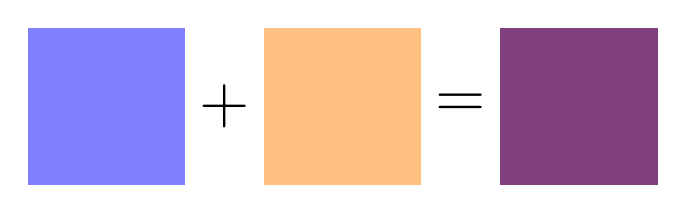
\begin{tikzpicture}
	\fill[blue!50] (0,0) rectangle (2,2);
	\node[black] (1) at (2.5,1) {\Huge{+}};
	\fill[orange!50] (3,0) rectangle (5,2);
	\node[black] (1) at (5.5,1) {\Huge{=}};
	\fill[blue!50!orange] (6,0) rectangle (8,2);
\end{tikzpicture}
\end{center}

\begin{Verbatim}[fontsize=\small]
\fill[blue!50!orange] (0,0) rectangle (2,2);
\end{Verbatim}
Når vi skriver 
\begin{Verbatim}[fontsize=\small]
\fill[blue!50] (0,0) rectangle (2,2);
\end{Verbatim}
så blander vi 50\% blå med 50\% hvit.

\newpage

% Plotte funksjoner
\subsection{Plotte funksjoner}
Man kan også plotte funksjoner i \TikZ. Da er det kjekt å kjenne til de forskjellige typer piler.

\begin{figure}[h!]
\centering
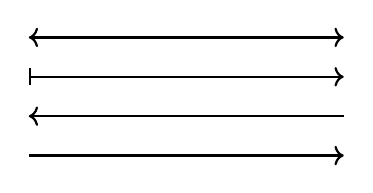
\begin{tikzpicture}
    \draw[->, thick] (0,0) -- (4,0);
    \draw[<-, thick] (0,0.5) -- (4,0.5);
    \draw[|->, thick] (0,1) -- (4,1);
    \draw[<->, thick] (0,1.5) -- (4,1.5);
\end{tikzpicture}
\caption{Piler i TikZ.}
\end{figure}

\begin{Verbatim}[fontsize=\small, frame=single]
\draw[<->] (0,1.5) -- (4,1.5);
\draw[|->] (0,1) -- (4,1);
\draw[<-]  (0,0.5) -- (4,0.5);
\draw[->]  (0,0) -- (4,0);
\end{Verbatim}

% plot
\subsubsection{\texttt{plot}}
\begin{center}
\scalebox{1.2}{
\begin{tikzpicture}
    \draw[<->] (0,3.5) -- (0,0) -- (5,0);
	\draw[red, thick, domain=0:1.2] plot (\x, {0.25+\x+\x*\x});
\end{tikzpicture}
}
\end{center}

\begin{Verbatim}[fontsize=\small, frame=single]
\begin{tikzpicture}
    \draw[<->] (0,3.5) -- (0,0) -- (5,0);
    \draw[red, thick, domain=0:1.2] plot (\x, {0.25+\x+\x*\x});
\end{tikzpicture}
\end{Verbatim}

\texttt{domain} er rekkevidden av $x$ som blir plottet. I dette tilfellet plotter vi funksjonen $0.25 + x + x^2$. Legg merke til at det er parenteser rundt funksjonen som vi skal plotte \texttt{plot (\textbackslash x, \{function\})}.

\vspace{10pt}

\Oppgave
\noindent Hvordan kan vi plotte dette
\scalebox{0.1}{
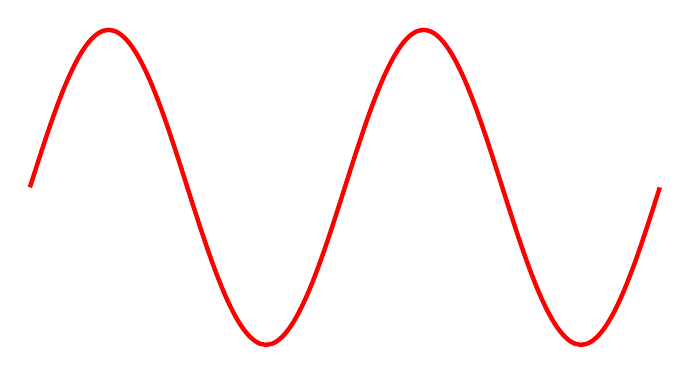
\begin{tikzpicture}
\draw[red, ultra thick] (0,0) sin (1,2) cos (2,0) sin (3,-2) cos (4,0) sin (5,2) cos (6,0) sin (7,-2) cos (8,0);
\end{tikzpicture}
}
?

\newpage

%%% KOORDINATER %%%
\section{Koordinatsystem}
Dette eksempelet krever et rutenett, piler, noder og plassering av tall og bokstaver. Vi starter med et rutenett:

\begin{center}
\scalebox{0.8}{
\begin{tikzpicture}
    \draw[step=1cm,gray!80,very thin] (-1.9,-1.9) grid (5.9,5.9);
\end{tikzpicture}
}
\end{center}

\begin{Verbatim}[fontsize=\small]
\draw[step=1cm,gray!80,very thin] (-1.9,-1.9) grid (5.9,5.9);
\end{Verbatim}

% Akser
\subsection{Akser}
\noindent Videre trenger vi x-aksen og y-aksen. Dette er to linjer med piler i enden.

\begin{center}
\scalebox{0.8}{
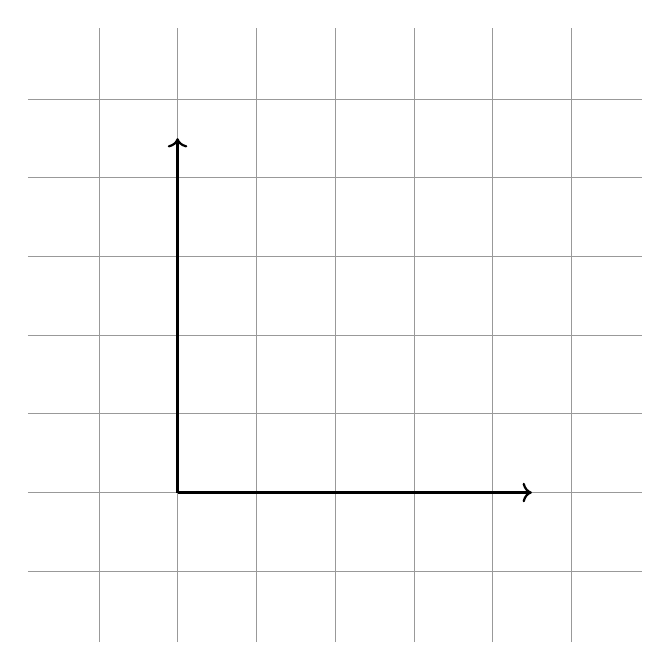
\begin{tikzpicture}
    \draw[step=1cm,gray!80,very thin] (-1.9,-1.9) grid (5.9,5.9);
    \draw[thick, ->] (0,0) -- (4.5,0);
    \draw[thick, ->] (0,0) -- (0,4.5);
\end{tikzpicture}
}
\end{center}

\begin{Verbatim}[fontsize=\small]
\draw[thick, ->] (0,0) -- (4.5,0);
\draw[thick, ->] (0,0) -- (0,4.5);
\end{Verbatim}

\newpage

% Noder
\subsection{Noder}
Vi kan legge på tekst (\textit{label}) ved å bruke nøkkelordet \texttt{node}. Vi plasserer teksten ved linjene vi har tegnet ved å fortelle noden hvor vi vil ha den.

\begin{center}
\scalebox{0.6}{
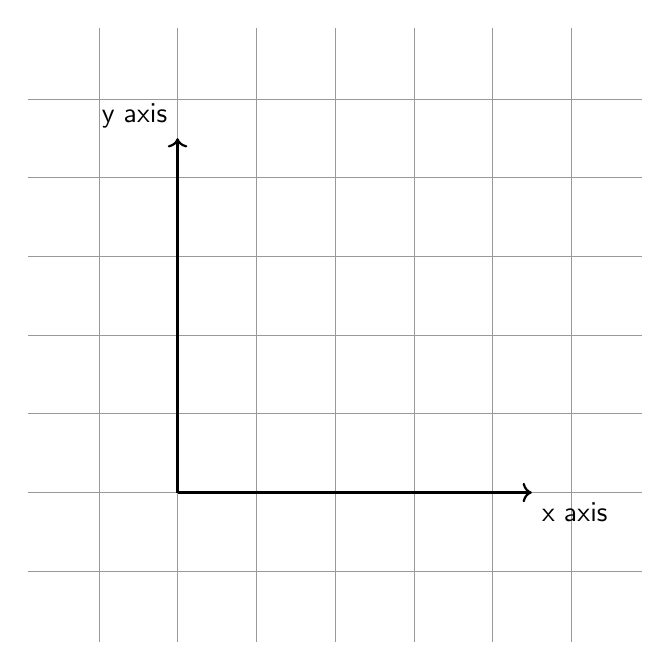
\begin{tikzpicture}
    \draw[step=1cm,gray!80,very thin] (-1.9,-1.9) grid (5.9,5.9);
    \draw[thick, ->] (0,0) -- (4.5,0) node[below right] {x axis};
    \draw[thick, ->] (0,0) -- (0,4.5) node[above left] {y axis};
\end{tikzpicture}
}
\end{center}

\begin{Verbatim}[fontsize=\small]
\draw[thick, ->] (0,0) -- (4.5,0) node[below right] {x axis};
\draw[thick, ->] (0,0) -- (0,4.5) node[above left] {y axis};
\end{Verbatim}

% Løkker
\subsection{Løkker}
\noindent Vi kan fortsette med tallene som skal gå langs aksene ved å bruke løkker:
\begin{center}
\scalebox{0.6}{
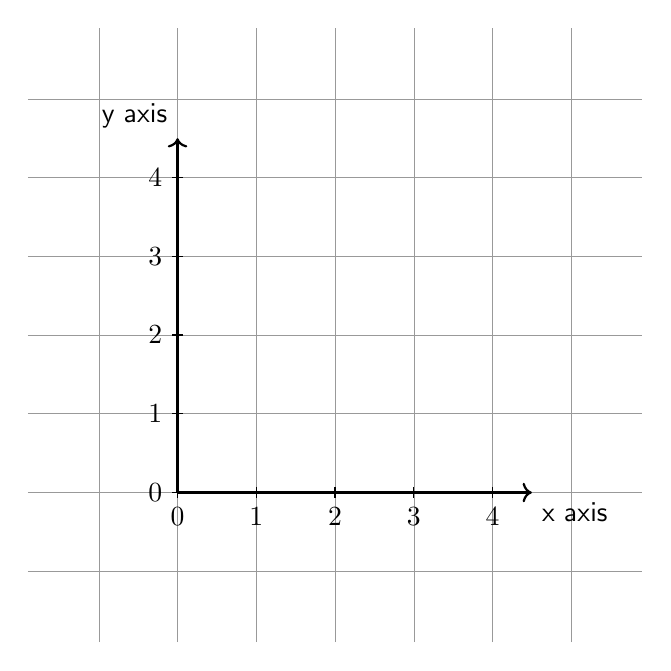
\begin{tikzpicture}
    \draw[step=1cm,gray!80,very thin] (-1.9,-1.9) grid (5.9,5.9);
    \draw[thick, ->] (0,0) -- (4.5,0) node[below right] {x axis};
    \draw[thick, ->] (0,0) -- (0,4.5) node[above left] {y axis};

    \foreach \x in {0,1,2,3,4}
	\draw (\x cm, 2pt) -- (\x cm, -2pt) node[below] {$\x$};
    \foreach \y in {0,1,2,3,4}
	\draw (2pt, \y cm) -- (-2pt, \y cm) node[left] {$\y$};
\end{tikzpicture}
}
\end{center}
Denne løkken går over linjene vi allerede har tegnet, og setter en liten strek for hver centimeter. Og ved siden av linjen skriver vi et tall.

\begin{Verbatim}[fontsize=\small, frame=single]
\foreach \x in {0,1,2,3,4}
  \draw (\x cm, 2pt) -- (\x cm, -2pt) node[below] {$\x$};
\foreach \y in {0,1,2,3,4}
  \draw (2pt, \y cm) -- (-2pt, \y cm) node[left]  {$\y$};
\end{Verbatim}
\Oppgave
Hvordan kan vi bruke \texttt{foreach} til å tegne dette
\scalebox{0.4}{
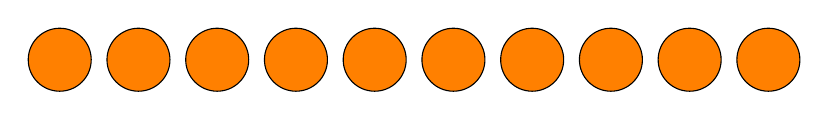
\begin{tikzpicture}
\foreach \x in {1,...,10}
	\draw[fill=orange] (\x, 0) circle (0.4cm);
\end{tikzpicture}
}
?

\subsection{Hele koden for koordinatsystemet}
\begin{center}
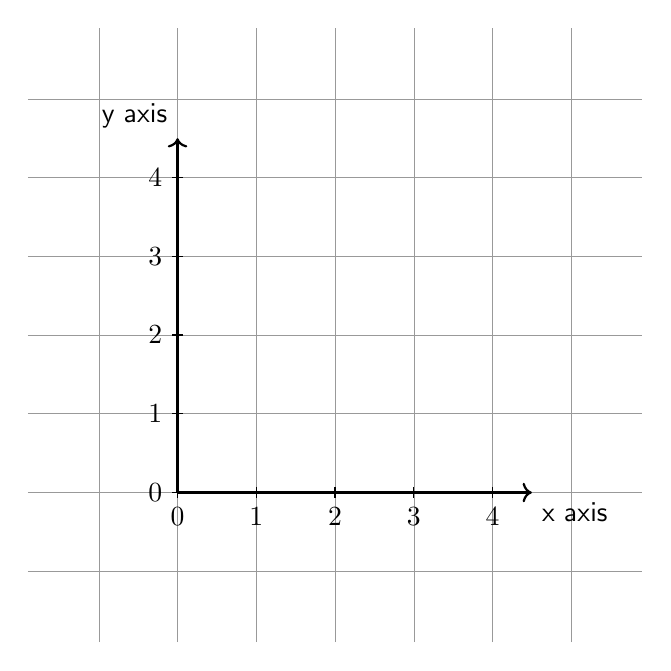
\begin{tikzpicture}
    \draw[step=1cm,gray!80,very thin] (-1.9,-1.9) grid (5.9,5.9);
    \draw[thick, ->] (0,0) -- (4.5,0) node[below right] {x axis};
    \draw[thick, ->] (0,0) -- (0,4.5) node[above left] {y axis};

    \foreach \x in {0,1,2,3,4}
	\draw (\x cm, 2pt) -- (\x cm, -2pt) node[below] {$\x$};
    \foreach \y in {0,1,2,3,4}
	\draw (2pt, \y cm) -- (-2pt, \y cm) node[left] {$\y$};
\end{tikzpicture}
\end{center}

\begin{Verbatim}[fontsize=\small, frame=single]
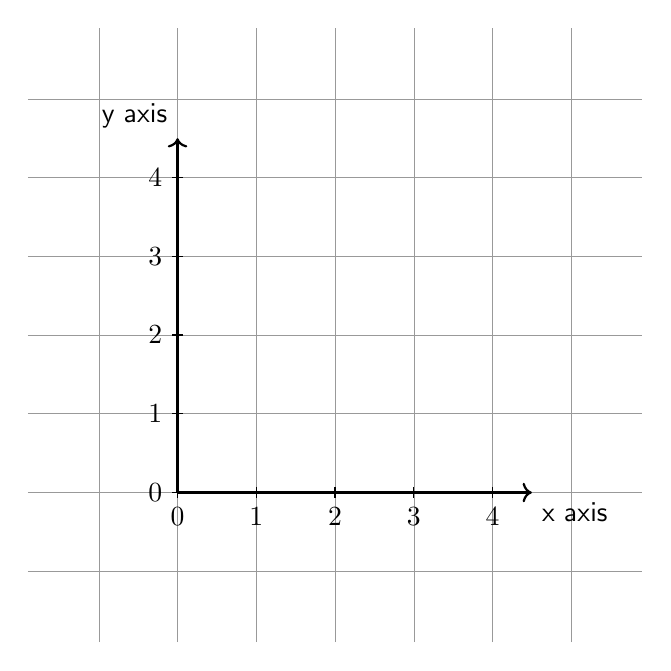
\begin{tikzpicture}
  \draw[step=1cm,gray!80,very thin] (-1.9,-1.9) grid (5.9,5.9);
  \draw[thick, ->] (0,0) -- (4.5,0) node[below right] {x axis};
  \draw[thick, ->] (0,0) -- (0,4.5) node[above left] {y axis};

  \foreach \x in {0,1,2,3,4}
    \draw (\x cm, 2pt) -- (\x cm, -2pt) node[below] {$\x$};
  \foreach \y in {0,1,2,3,4}
    \draw (2pt, \y cm) -- (-2pt, \y cm) node[left] {$\y$};
\end{tikzpicture}
\end{Verbatim}

\Oppgave
\noindent Hvordan kan vi tegne dette?

\begin{center}
\scalebox{0.7}{
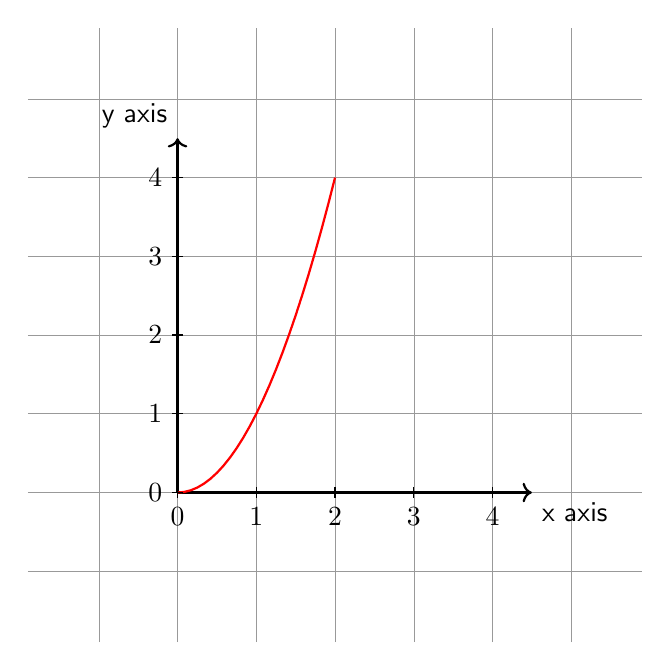
\begin{tikzpicture}
    \draw[step=1cm,gray!80,very thin] (-1.9,-1.9) grid (5.9,5.9);
    \draw[thick, ->] (0,0) -- (4.5,0) node[below right] {x axis};
    \draw[thick, ->] (0,0) -- (0,4.5) node[above left] {y axis};
 	\draw[red, thick, domain=0:2] plot (\x, {\x*\x});

    \foreach \x in {0,1,2,3,4}
	\draw (\x cm, 2pt) -- (\x cm, -2pt) node[below] {$\x$};
    \foreach \y in {0,1,2,3,4}
	\draw (2pt, \y cm) -- (-2pt, \y cm) node[left] {$\y$};
\end{tikzpicture}
}
\end{center}

\newpage

%%% TRÆR %%%
\section{Trær}
Et tre består av en rekke noder. Når vi tegner trær i \TikZ starter vi med å definere rot-noden. Legg merke til attributtene vi gir \texttt{tikzpicture}. Her sier vi at \texttt{every node} skal ha \textit{stilen} (\texttt{.style}) sirkel med sort strek.

\begin{center}

\begin{tikzpicture}[every node/.style={circle, draw=black},level 2/.style={sibling distance=20mm},
				   level 3/.style={sibling distance=10mm}, level distance=30pt]
\node {1};
\end{tikzpicture}
\end{center}

\begin{Verbatim}[fontsize=\small, frame=single]

\begin{tikzpicture}[every node/.style={circle, draw=black}]
    \node {1};
\end{tikzpicture}
\end{Verbatim}

\subsection{Bygge treet}
Treet bygger vi ved å legge til barna. Barna skrives på formen:
\begin{Verbatim}[fontsize=\small]
child { node[opt.] {value} }
\end{Verbatim}

\begin{center}
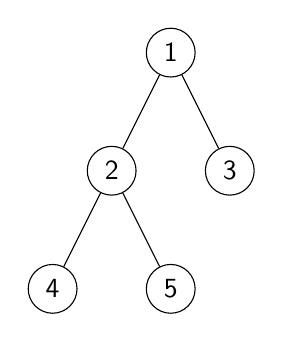
\begin{tikzpicture}[every node/.style={circle, draw=black}]
\node {1}
	child { node {2} 
		child { node {4} }
		child { node {5} }
	}
	child { node {3} }
;
\end{tikzpicture}
\end{center}

\begin{Verbatim}[fontsize=\small, frame=single]
\node {1}
    child { node {2} 
        child { node {4} }
        child { node {5} }
    }
    child { node {3} }
;
\end{Verbatim}
\texttt{[opt.]} i definisjonen av \texttt{node} sier noe om hvordan noden skal se ut. Her kan vi for eksempel skrive \texttt{node[red]}, så får vi at denne ene noden skal være rød. 

\newpage

\subsection{Justere avstand mellom noder}

Når vi nå vil bygge videre og legge til tallet 6 under \texttt{child \{node \{3\}\}} vil vi overlappe 5. Da trenger vi å justere avstanden mellom søsken-noder.

\vspace{20pt}

\begin{minipage}{0.5\textwidth}
Vi har: \newline \newline
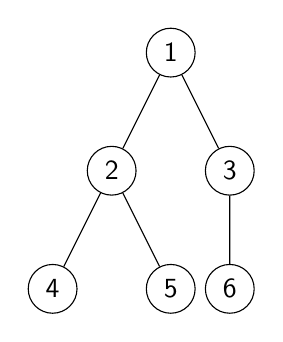
\begin{tikzpicture}[every node/.style={circle, draw=black}]
\node {1}
	child { node {2} 
		child { node {4} }
		child { node {5} }
	}
	child { node {3} 
		child { node {6} }
	}
;
\end{tikzpicture}
\end{minipage}
\begin{minipage}{0.5\textwidth}
Vi vil ha: \newline \newline
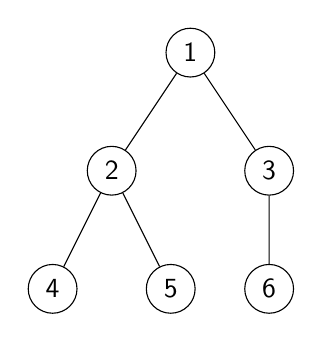
\begin{tikzpicture}[every node/.style={circle, draw=black}, 
				   level 1/.style={sibling distance=20mm}, 
				   level 2/.style={sibling distance=15mm}]
\node {1}
	child { node {2} 
		child { node {4} }
		child { node {5} }
	}
	child { node {3} 
		child {node {6} }
	}
;
\end{tikzpicture}
\end{minipage}

\vspace{20pt}

Da legger vi på et attributt til i listen til \texttt{tikzpicture} som forteller noe om avstanden mellom nodene. 

\begin{Verbatim}[fontsize=\small, frame=single]
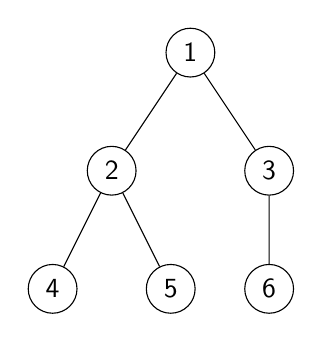
\begin{tikzpicture}[every node/.style={circle, draw=black}, 
		    level 1/.style={sibling distance=20mm}, 
		    level 2/.style={sibling distance=15mm}]

\node {1}
    child { node {2} 
        child { node {4} }
        child { node {5} }
    }
    child { node {3} 
        child {node {6} }
    }
;
\end{tikzpicture}
\end{Verbatim}

Her forteller vi at stilen til nodene på \texttt{level 1} skal være at de har avstand til sine søsken med 20 mm, og 15 mm for \texttt{level 2}. Vi kunne også lagt til attributtet \texttt{level distance} for å få større eller mindre avstand mellom lagene. 

\newpage

% Fasonger på noder
\subsection{Fasonger som noder kan ha}
Man kan få forskjellige fasonger på noder ved å inkludere \texttt{\textbackslash usetikzlibrary\{shapes\}}. Her er en oversikt over forskjellige fasonger en node kan ha. For å få ønsket fasong skriver man noden på denne formen:
\begin{Verbatim}[fontsize=\small, frame=single]
\node[rectangle] {Rectangle};
\node[regular polygon, regular polygon sides=5] {n=5};
\node[circle split] {Circle \nodepart{lower} split};
\end{Verbatim}

\begin{figure}[h!]
\centering
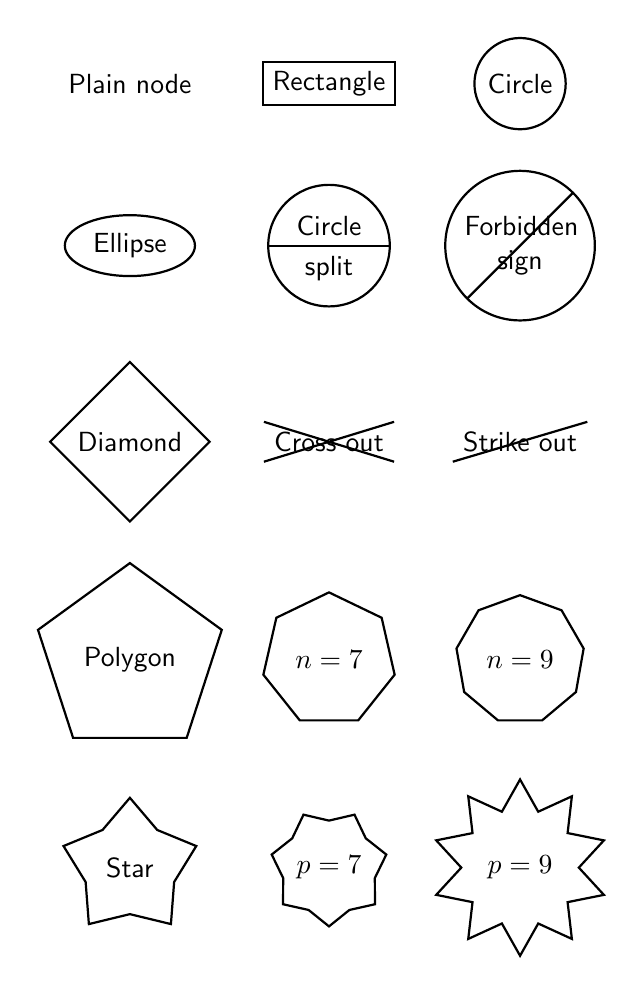
\begin{tikzpicture}
    \matrix[nodes={draw, thick},
        row sep=0.5cm,column sep=0.5cm] {
    \node[draw=none,fill=none] {Plain node}; &
    \node[rectangle] {Rectangle}; &
    \node[circle] {Circle};\\
    \node[ellipse] {Ellipse};&
    \node[circle split] {Circle \nodepart{lower} split};&
    \node[forbidden sign,text width=4em, text centered] {Forbidden sign};\\
    \node[diamond] {Diamond};&
    \node[cross out] {Cross out};&
    \node[strike out] {Strike out};\\
    \node[regular polygon,regular polygon sides=5] {Polygon};&
    \node[regular polygon,regular polygon sides=7] {$n=7$};&
    \node[regular polygon,regular polygon sides=9] {$n=9$};\\
    \node[star] {Star};&
    \node[star,star points=7,star point ratio=0.8] {$p=7$};&
    \node[star,star points=10] {$p=9$};\\
    };
\end{tikzpicture}
\caption{Fasonger på noder.}
\end{figure}

\newpage

\subsection{Eksempel på et tre med avstander}

\begin{center}
\begin{tikzpicture}[every node/.style={},level 2/.style={sibling distance=20mm},
				   level 3/.style={sibling distance=10mm}, level distance=30pt]
\node {S}
	child { node{A} 
		child { node {A} 
			child { node {(} }
			child { node {)} }
		}
		child { node {A} 
			child { node {(} }
			child { node {A} 
				child { node {(} }
				child { node {)} }
			}
			child { node {)} }
		}
	};
\end{tikzpicture}
\end{center}

\begin{Verbatim}[fontsize=\small, frame=single]
\begin{tikzpicture}[every node/.style={},
                    level 2/.style={sibling distance=20mm},
                    level 3/.style={sibling distance=10mm}, 
                    level distance=30pt]
\node {S}
    child { node{A} 
        child { node {A} 
            child { node {(} }
            child { node {)} }
        }
        child { node {A} 
            child { node {(} }
            child { node {A} 
                child { node {(} }
                child { node {)} }
            }
            child { node {)} }
        }
    }
;
\end{tikzpicture}
\end{Verbatim}

\newpage

\subsection{Rød-svarte trær}

\tikzset{
	treenode/.style = {align=center, inner sep=0pt},
	% Sorte noder
  	node_black/.style = {treenode, circle, white, font=\bfseries, draw=black,fill=black, text width=0.8cm},
	% Røde noder
  	node_red/.style = {treenode, circle, red, draw=red, text width=0.8cm, very thick},
	% Null-pekere
  	node_null/.style = {treenode, rectangle, draw=black, minimum width=0.3cm, minimum height=0.3cm}
}
\begin{center}
% Skal tegne med piler (->), og setter level/.style={opt.} %
\begin{tikzpicture}[->,level/.style={sibling distance = 2cm, level distance = 1.5cm}] 
\node [node_black] {38}
    	child{ node [node_red] {19} 
		child{node [node_black] {12}
			child{node [node_red] {8}}
			child{node [node_null] {}}
		}
		child{node [node_black] {31}}
	}
    	child{ node [node_black] {41} }
; 
\end{tikzpicture}
\end{center}

Å tegne trær på denne måten krever ingen tilleggsbiblioteker fra \TikZ. Dette er et eksempel på tegning med egendefinerte noder. Dette gjør vi via \texttt{tikzset}, her kan vi gi stilen de forskjellige typene noder.
\begin{Verbatim}[fontsize=\small, frame=single]
\tikzset{
   treenode/.style = {align=center},
	
   % Sorte noder
   node_black/.style = {treenode, circle, white, 
			font=\bfseries, draw=black,
			fill=black, text width=0.8cm},
   % Røde noder
   node_red/.style = {treenode, circle, red, draw=red, 
	              text width=0.8cm, very thick},
   % Null-pekere
   node_null/.style = {treenode, rectangle, draw=black, 
		       minimum width=0.3cm, minimum height=0.3cm}
}
\end{Verbatim}
Starter med å definere \texttt{treenode}, som er felles for alle nodene. Røde og sorte noder tegnes som \texttt{circle}, hvor sorte noder har \texttt{fill=black} og tekstfarge \texttt{white}, mens røde noder har rødt omriss med \texttt{draw=red}, og tekstfarge \texttt{red}. Null-nodene sier vi skal være sorte \texttt{rectangle}. Tegnes som små kvadrater på 0.3 cm $\times$ 0.3 cm.

\newpage
\subsection{Bygge det rød-svarte treet}
\begin{Verbatim}[fontsize=\small, frame=single]
\begin{tikzpicture}[->,level/.style={ sibling distance = 2cm, 
                    level distance = 1.5cm }] 
\node [node_black] {38}
    child { node [node_red] {19} 
        child { node [node_black] {12}
             child { node [node_red] {8} }
             child { node [node_null] {} }
        }
        child { node [node_black] {31} }
    }
    child { node [node_black] {41} }
; 
\end{tikzpicture}
\end{Verbatim}

Setter forskjellige opsjoner med:
\begin{Verbatim}[fontsize=\small, frame=single]
\begin{tikzpicture}[->,level/.style={ sibling distance = 2cm, 
                    level distance = 1.5cm }]
\end{Verbatim}
Her sier vi at treet skal tegnes med piler (\texttt{->}), og at stilen (\texttt{.style}) for distansen mellom søskennoder skal være 2 cm, og distansen mellom barn og foreldre skal være 1.5 cm.

Videre så forteller vi barna i treet hva slags node de skal være.
\begin{Verbatim}[fontsize=\small, frame=single]
child { node [node_red]   {x} }
child { node [node_black] {y} }
child { node [node_null]  {z} }
\end{Verbatim}

\vspace{25pt}

\Oppgave
\noindent Hvordan kan vi tegne dette treet?
\tikzset{
	treenode/.style = {align=center, inner sep=0pt},
  	star_node/.style = {treenode, star, black,fill=yellow, text width=0.5cm},
	star_node_super/.style = {treenode, star, star points=9, white, fill=orange, font=\bfseries, text width=0.8cm},
}
\begin{center}
\begin{tikzpicture}[->,level/.style={ sibling distance = 2cm, 
                    level distance = 3cm }] 
\node [star_node_super] {1}
    child { node [star_node] {2} }
    child { node [star_node] {3} }
    child { node [star_node] {4} }
; 
\end{tikzpicture}
\end{center}

\newpage

%%% GRAFER %%%
\section{Grafer}

\begin{center}
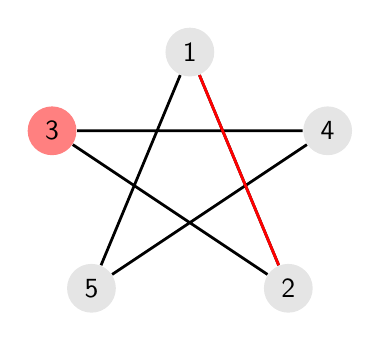
\begin{tikzpicture}[scale=5]
	 \tikzstyle{vertex}=[circle,fill=black!10]
	 \tikzstyle{selected vertex} = [vertex, fill=red!50]

	 \tikzstyle{selected edge} = [draw,line width=1pt,-,red!100]
	 \tikzstyle{edge} = [-,black,line width=1pt]

	 \node[vertex] (v1) at (1.25,1.7) 			{1};
	 \node[vertex] (v2) at (1.5,1.1) 				{2};
	 \node[selected vertex] (v3) at (0.9,1.5) 		{3};
	 \node[vertex] (v4) at (1.6,1.5) 				{4};
	 \node[vertex] (v5) at (1,1.1) 				{5};

	\draw[edge] (v1)  -- (v2) -- (v3) -- (v4) -- (v5) -- (v1); 
	\draw[selected edge] (v1) -- (v2);
\end{tikzpicture}
\end{center}
Det fins enklere måter å tegne grafer på enn dette, men jeg syns denne måten er fin. Den krever heller ingen andre biblioteker eller pakker enn \TikZ selv. 

Vi starter med å definere de forskjellige elementene til en graf.

\begin{Verbatim}[fontsize=\small, frame=single]
\begin{tikzpicture}
    \tikzstyle{vertex} = [circle,fill=black!10]
    \tikzstyle{selected vertex} = [vertex, fill=red!50]

    \tikzstyle{selected edge} = [draw,line width=1pt,-,red!100]
    \tikzstyle{edge} = [-,black,line width=1pt]
\end{tikzpicture}
\end{Verbatim}
Her forteller vi at \texttt{vertex}er (eller noder), skal være sirkler. Markerte noder skal være fylt med rød farge.
\begin{center}

\begin{tikzpicture}[scale=2]
	 \tikzstyle{vertex}=[circle,fill=black!10]
	 \tikzstyle{selected vertex} = [vertex, fill=red!50]

	 \node[vertex] (v1) at (1,1) 				{1};
	 \node[selected vertex] (v2) at (2,1) 		{2};
\end{tikzpicture}
\end{center}

\noindent Kanter skal tegnes som sorte linjer (\texttt{[-, black $\dots$]}). Og markerte kanter skal være røde.

\begin{center}
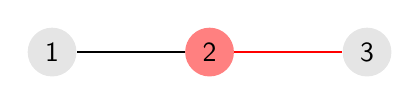
\begin{tikzpicture}[scale=2]
	 \tikzstyle{vertex}=[circle,fill=black!10]
	 \tikzstyle{selected vertex} = [vertex, fill=red!50]
	 \tikzstyle{selected edge} = [draw,line width=1pt,-,red!100]
	 \tikzstyle{edge} = [-,black,line width=1pt]

	 \node[vertex] (v1) at (1,1) 				{1};
	 \node[selected vertex] (v2) at (2,1) 		{2};
	\node[vertex] (v3) at (3,1)					{3};
	\draw[edge] (v1) -- (v2);
	\draw[selected edge] (v2) -- (v3);
\end{tikzpicture}
\end{center}

\newpage
\subsection{Tegne grafen} 
For å plassere nodene rundt om på arket sier man hvor man vil de skal være ved hjelp av koordinater.

\begin{Verbatim}[fontsize=\small, frame=single]
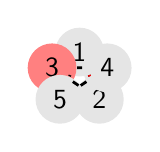
\begin{tikzpicture}
    \tikzstyle{vertex}          = [circle,fill=black!10]
    \tikzstyle{selected vertex} = [vertex, fill=red!50]

    \tikzstyle{selected edge}   = [draw,line width=1pt,-,red!100]
    \tikzstyle{edge}            = [-,black,line width=1pt]

    \node[vertex]          (v1) at (1.25,1.7) {1};
    \node[vertex]          (v2) at (1.5,1.1)  {2};
    \node[selected vertex] (v3) at (0.9,1.5)  {3};
    \node[vertex]          (v4) at (1.6,1.5)  {4};
    \node[vertex]          (v5) at (1,1.1)    {5};

    \draw[edge]          (v1)--(v2)--(v3)--(v4)--(v5)--(v1); 
    \draw[selected edge] (v1)--(v2);
\end{tikzpicture}
\end{Verbatim}

% Noder
\subsection{Noder} 
Nodene defineres ved å først bruke nøkkelordet \texttt{node}, så fortelle hvilken type node dette er. I dette tilfellet, så er det enten \texttt{vertex} eller \texttt{selected vertex} som vi har definert med \texttt{tikzstyle}. Nodens navn bruker man kun i egen kode, når vi skal tegne opp kantene trenger vi disse navnene. Koordinatene \texttt{(x,y)} forteller hvor vi vil plassere noden, og verdien er innholdet i noden.
\begin{Verbatim}[fontsize=\small]
\node[type of node] (node name) at (x,y) {value};
\end{Verbatim}

% Kanter
\subsection{Kanter}
Kantene tegnes likt som linjer fra seksjon 1. Men her gir vi nøkkelordet \texttt{draw} en av to stiler, som vi definerte med \texttt{tikzstyle}. Enten \texttt{edge} eller \texttt{selected egde}.

\begin{Verbatim}[fontsize=\small]
\draw[type of edge] (from node) -- (to node);
\end{Verbatim}

\Oppgave
\noindent Hvordan kan vi tegne denne?
\begin{center}
\scalebox{0.2}{
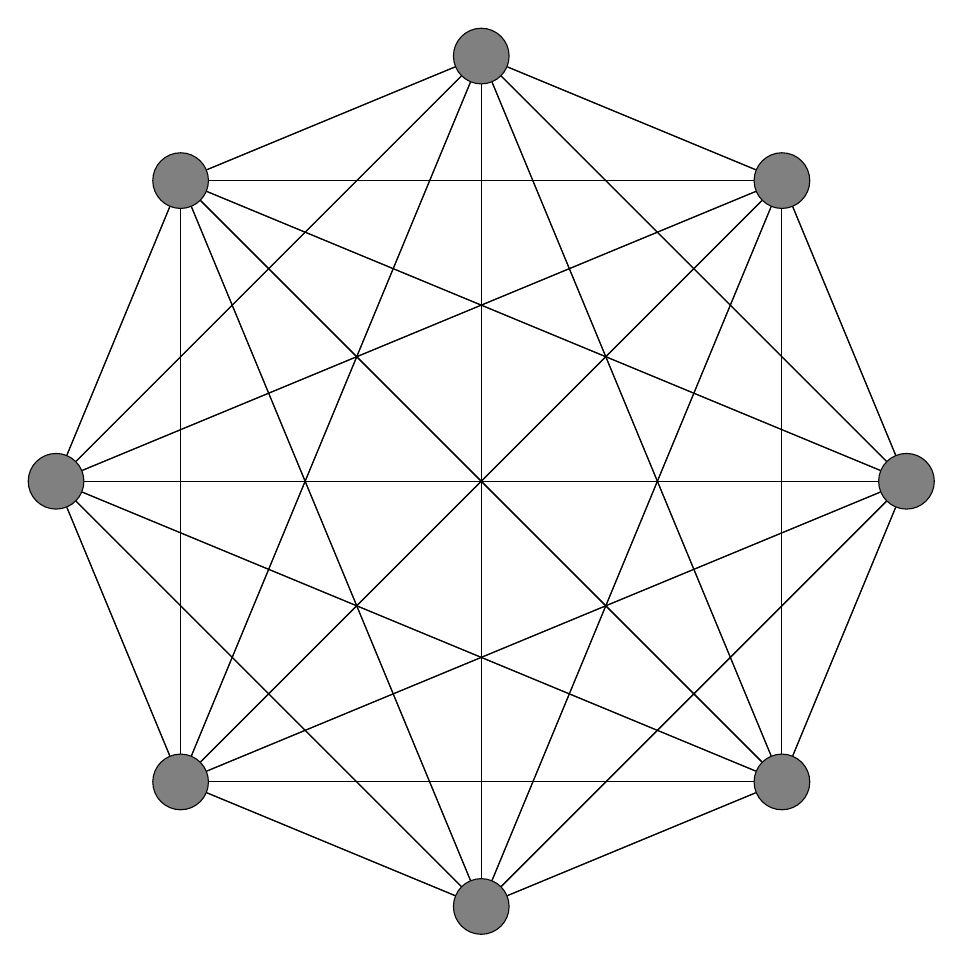
\begin{tikzpicture}
\foreach \x in {1,...,8}{%
	\pgfmathparse{(\x-1)*360/8}
	\node[draw,circle,inner sep=0.25cm, fill=gray] (N-\x) at (\pgfmathresult:5.4cm) {};
}
\foreach \x in {1,...,8}{%
	\foreach \y in {1,...,8}{%
		\path (N-\x) edge[black,-] (N-\y);
	}
}
\end{tikzpicture}
}
\end{center}

\newpage

%%% AUTOMATER %%%
\section{Automater}
Denne måten å tegne automater på krever at man inkluderer et \TikZ-bibliotek.
\begin{Verbatim}[fontsize=\small]
\usetikzlibrary{automata}
\end{Verbatim}

\begin{center}
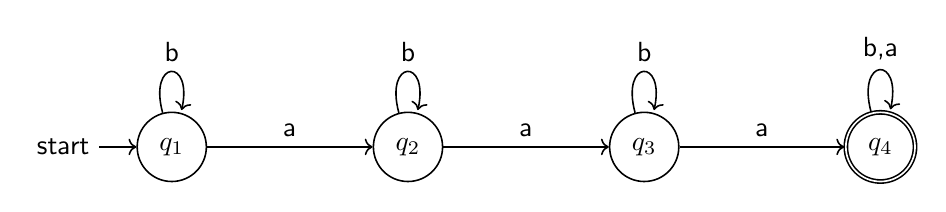
\begin{tikzpicture}[->,auto,node distance=3cm,line width=0.2mm]
  \node[initial,state] 			(A)		 	         {$q_1$};
  \node[state]         			(B) [right of=A] 	{$q_2$};
  \node[state]				(C) [right of=B] 	{$q_3$};
  \node[state,accepting]		(D) [right of=C] 	{$q_4$};

  \path 	(A) edge [loop above] node 			{b} 		(A)
			edge node 						{a} 		(B)
        		(B) edge [loop above] node 			{b} 		(B)
			edge node 						{a} 		(C)
		(C) edge [loop above] node 			{b}		(C)
			edge node 						{a} 		(D)
		(D) edge [loop above] node 			{b,a}	(D);
\end{tikzpicture}
\end{center}

\begin{Verbatim}[fontsize=\small, frame=single]
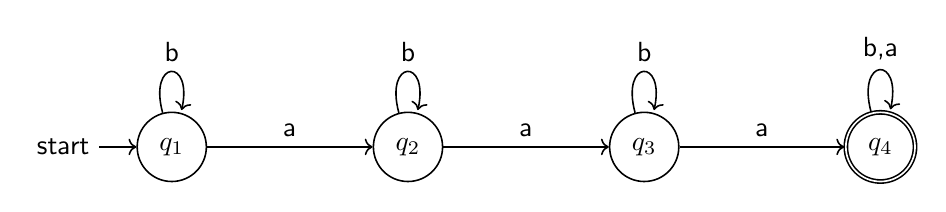
\begin{tikzpicture}[->,auto,node distance=3cm,line width=0.2mm]
  \node[initial,state]  (A) 		{$q_1$};
  \node[state]          (B) [right of=A]    {$q_2$};
  \node[state]	  (C) [right of=B]    {$q_3$};
  \node[state,accepting](D) [right of=C]    {$q_4$};

  \path (A) edge [loop above] node 	 {b}   (A)
	    edge node      		 {a}   (B)
        (B) edge [loop above] node 	 {b}   (B)
	    edge node   	  	  {a}   (C)
        (C) edge [loop above] node	  {b}   (C)
	    edge node 	    	  {a}   (D)
        (D) edge [loop above] node 	 {b,a} (D);
\end{tikzpicture}
\end{Verbatim}
For denne måten å tegne automater på, så settes alle attributter som beskriver automaten i definisjonen til \texttt{tikzpicture}. 
Her har automaten følgende egenskaper:
\begin{center}
\texttt{\{tikzpicture\}[->, auto, node distance=3cm, line width=0.2mm]}
\end{center}
Dette forteller oss at automaten skal tegnes med piler (\texttt{->}), nodene skal ha avstand på 3 cm, og linjene en tykkelse på 0,2 mm. \texttt{auto} stiller teksten \textit{over} linjene, i stedet for \textit{på} linjene.

\subsection{Automatens tilstander} En automat har tre typer tilstander: starttilstanden, vanlig tilstand(er), og akepterende tilstand(er).

\begin{Verbatim}[fontsize=\small]
\node[state] (node name) {state name};
\end{Verbatim}

I tillegg til \texttt{[state]}, så kan man ha med opsjonen \texttt{[initial, state]} for starttilstanden, eller \texttt{[state, accepting]} for aksepterende tilstand.

\subsection{Stien gjennom automaten}
Stien tegnes gjennom en \texttt{path}. Denne konstrueres på følgende vis:

\begin{Verbatim}[fontsize=\small]
\path (from state) edge [opt.] node {weight} (to state)
\end{Verbatim}

\noindent Her kan \texttt{[opt]} være \texttt{loop above/below}, \texttt{bend left/right}.

\subsection*{Flittig bever}
Her er en flittig 4-bever. Denne automaten dekker de fleste opsjoner.
\begin{center}
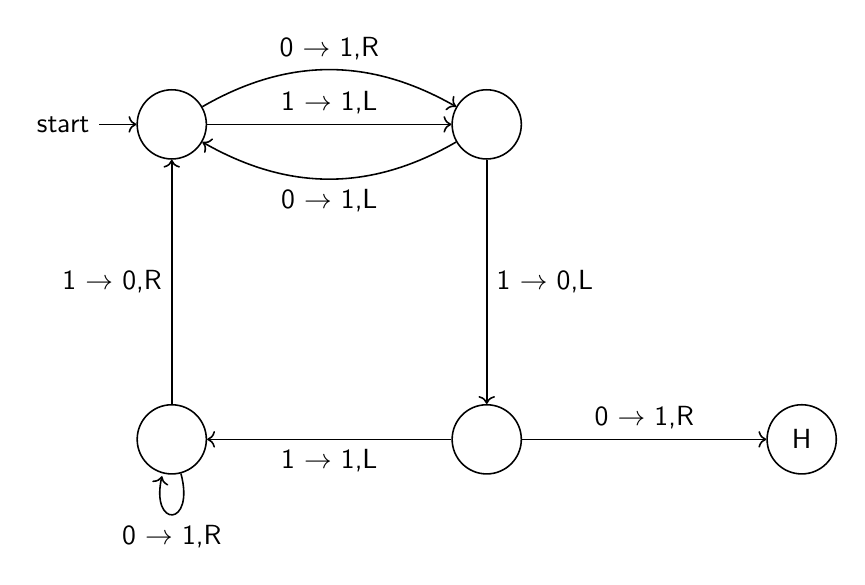
\begin{tikzpicture}[->,auto,node distance=4cm,line width=0.2mm]
  \node[initial,state] 		(A)            			{};
  \node[state] 			(B) [below of=A]   	{};
  \node[state] 			(C) [right of=A]    		{};
  \node[state] 			(D) [below of=C] 		{};
  \node[state]         		(E) [right of=D] 		{H};

  \path 	(A) edge node 				{1 $\rightarrow$ 1,L} 		(C)
		(A) edge [bend left] node 		{0 $\rightarrow$ 1,R} 		(C)
		(C) edge [bend left] node 		{0 $\rightarrow$ 1,L} 		(A)
		(B) edge node 				{1 $\rightarrow$ 0,R} 		(A)
		(B) edge [loop below] node 	{0 $\rightarrow$ 1,R} 		(B)
		(D) edge node 				{1 $\rightarrow$ 1,L} 		(B)
		(C) edge node 				{1 $\rightarrow$ 0,L} 		(D)
		(D) edge node		 		{0 $\rightarrow$ 1,R} 		(E);
\end{tikzpicture}
\end{center}

\begin{Verbatim}[fontsize=\small, frame=single]
\begin{tikzpicture}[->,auto,node distance=4cm,line width=0.2mm]
  \node[initial,state] (A)              {};
  \node[state] 	(B) [below of=A] {};
  \node[state] 	(C) [right of=A] {};
  \node[state] 	(D) [below of=C] {};
  \node[state]         (E) [right of=D] {H};

  \path (A) edge node   	   {1 $\rightarrow$ 1,L}  (C)
	(A) edge [bend left] node  {0 $\rightarrow$ 1,R}  (C)
	(C) edge [bend left] node  {0 $\rightarrow$ 1,L}  (A)
	(B) edge node 	     {1 $\rightarrow$ 0,R}  (A)
	(B) edge [loop below] node {0 $\rightarrow$ 1,R}  (B)
	(D) edge node 	     {1 $\rightarrow$ 1,L}  (B)
	(C) edge node 	     {1 $\rightarrow$ 0,L}  (D)
	(D) edge node	      {0 $\rightarrow$ 1,R}  (E);
\end{tikzpicture}
\end{Verbatim}

\newpage

%%% ANDRE TIKZ BIBLIOTEKER %%%
\section{Forskjellige \TikZ biblioteker}
Som med automatene, er det flere andre \TikZ-biblioteker som kan inkluderes. Her kommer noen eksempler.

\subsection{\texttt{mindmap}}

\begin{center}
\scalebox{0.7}{
\begin{tikzpicture}
  \path[mindmap,concept color=violet,text=white]
    node[concept] {TikZ-kurs}
    [clockwise from=0]
    child[concept color=purple] {
      node[concept] {The Basics}
      [clockwise from=90]
      child { node[concept] {Fasonger} }
      child { node[concept] {Farger} }
    }  
    child[concept color=cyan] {
      node[concept] {Trær}
      [clockwise from=-30]
      child { node[concept] {Noder} 
		child { node[concept] {Egendefinerte noder}}
	}
      child { node[concept] {Justere avstand} }
    }
    child[concept color=red] { node[concept] {Automater} }
    child[concept color=orange] { node[concept] {Grafer} };
\end{tikzpicture}
}
\end{center}

\begin{Verbatim}[fontsize=\footnotesize, frame=single]
\path[mindmap,concept color=violet,text=white]
    node[concept] {TikZ-kurs}
    [clockwise from=0]
    child[concept color=purple] { 
    node[concept] {The Basics} [clockwise from=90]
        child { node[concept] {Fasonger} }
        child { node[concept] {Farger} }
    }  
    child[concept color=cyan] {
    node[concept] {Trær} [clockwise from=-20]
        child { node[concept] {Noder} 
            child { node[concept] {Egendefinerte noder}}
        }
        child { node[concept] {Justere avstand} }
     }
    child[concept color=red] { node[concept] {Automater} }
    child[concept color=orange] { node[concept] {Grafer} };
\end{Verbatim}

\newpage

\subsection{\texttt{calendar}}

\begin{center}
\begin{tikzpicture}[every day/.style={anchor=mid}]
\calendar (mycalendar) [dates=2014-10-01 to 2014-10-31,week list, 
					    month label above centered,
					    month text=\textcolor{teal}{\%mt} \%y-] 
					    if (Sunday) [red]
					    if (equals=2014-10-06) {\draw[red,thick] (0,0) circle (7pt);};
\end{tikzpicture}
\end{center}

\begin{Verbatim}[fontsize=\footnotesize, frame=single]
\begin{tikzpicture}
    \calendar (mycalendar) [dates=2014-10-01 to 2014-10-31,week list, 
                            month label above centered]
                            month text=\textcolor{teal}{\%mt} \%y-] 
                            if (Sunday) [red]
                            if (equals=2014-10-06) 
                               {\draw[red,thick] (0,0) circle (7pt);};
\end{tikzpicture}
\end{Verbatim}

\paragraph{Attributter} Attributter som vi gir kalenderen \texttt{mycalendar} er at den skal strekke seg fra 1. oktober 2014 til 31. oktober 2014. Den skal tegnes som lister av uker, og månedens navn skal skrives på toppen, sentrert. Vi sier også at tekstfargen til måneden skal være \textit{teal}, og at vi skal legge på året.

\paragraph{If-setninger} Her har vi også et eksempel på \texttt{if}-setninger i \TikZ. Disse er på formen
\begin{Verbatim}[fontsize=\footnotesize, frame=single]
if=(<condition>)<code or options> else<else code or options>
\end{Verbatim}

I dette eksempelet sier vi at \textit{hvis} dagen er en søndag, så skal teksten være rød. Og hvis datoen er 6. oktober 2014, så skal vi tegne en rød ring rundt denne.


\newpage

%%% LOGISKE PORTER %%%
\section{Circuitikz}
Noe som er kjekt å vite om er også logiske porter i Circuitikz. Dette får du ved å inkludere pakken:
\begin{Verbatim}[fontsize=\small]
\usepackage{circuitikz}
\end{Verbatim}
Siden dette \textit{ikke} er \TikZ jobber vi ikke i miljøet \texttt{tikzpicture}, men i miljøet \texttt{circuitikz}.

\begin{Verbatim}[fontsize=\small, frame=single]
\begin{circuitikz} \draw
    <kode her>
\end{circuitikz}
\end{Verbatim}

\subsection{Eksempel på en liten krets}

\begin{center}
\begin{circuitikz} \draw
(-3,0.3) node[not port] (not) {}
(0,0) node[and port] (and) {}
(2,1) node[or port] (or) {}
(not.out) -- (and.in 1)
(and.out) -- (or.in 2);
\end{circuitikz}
\end{center}

\begin{Verbatim}[fontsize=\small, frame=single]
\begin{circuitikz} \draw
    (-3,0.3) node[not port] (not) {}
    (0,0)    node[and port] (and) {}
    (2,1)    node[or port]  (or)  {}

    (not.out) -- (and.in 1)
    (and.out) -- (or.in 2);
\end{circuitikz}
\end{Verbatim}
Det fungerer på samme måte som når vi tegner noder i TikZ. Vi starter med koordinatene, så definerer vi hva slags node (port) vi vil ha, og til slutt en evt. merkelapp.

\begin{Verbatim}[fontsize=\small]
(x,y) node [what kind of port] (name of port) {label}
\end{Verbatim}
Portens navn er valgfritt, og brukes kun i din egen kode. 

\newpage

\subsection{Oversikt over forskjellige porter i Circuitikz}
\begin{figure}[h!]
\centering
\begin{tabular}{ll}
\texttt{[and port]} & \begin{circuitikz} \draw (0,0) node[and port] (myand1) {}; \end{circuitikz}\\
\texttt{[or port]} & \begin{circuitikz} \draw (0,0) node[or port] (myand1) {}; \end{circuitikz}\\
\texttt{[not port]} & \begin{circuitikz} \draw (0,0) node[not port] (myand1) {}; \end{circuitikz}\\
\texttt{[nand port]} & \begin{circuitikz} \draw (0,0) node[nand port] (myand1) {}; \end{circuitikz}\\
\texttt{[nor port]} & \begin{circuitikz} \draw (0,0) node[nor port] (myand1) {}; \end{circuitikz}\\
\texttt{[xor port]} & \begin{circuitikz} \draw (0,0) node[xnor port] (myand1) {}; \end{circuitikz}\\
\end{tabular}
\caption{Forskjellige porter i Circuitikz}
\end{figure}

\newpage

\section{Ressurser}
\subsection*{Gøyale eksempler}
\begin{itemize}
	\item
	\href{http://www.texample.net/tikz/examples/enderman/}{Enderman}

	\item
	\href{http://www.texample.net/tikz/examples/dartboard/}{Dartboard}

	\item
	\href{http://www.texample.net/tikz/examples/india-map/}{India map}
\end{itemize}

\subsection{Nyttige lenker}
\begin{itemize}
	\item
	\href{http://www.tug.org/TUGboat/tb30-2/tb95mertz.pdf}{A \TikZ tutorial: Generating graphics in the spirit of \TeX}
	\item
	\href{http://www.texample.net/media/pgf/builds/pgfmanualCVS2012-11-04.pdf}{\TikZ \& PGF Manual}
	\item
	\href{https://www.tug.org/pracjourn/2007-1/mertz/mertz.pdf}{Graphics with \TikZ}
	\item
	\href{http://www.texample.net/}{TeXample.net}
	\item
	\href{http://tug.org/}{\TeX Users Group (tug.org)}
\end{itemize}


\subsection*{Visste du at..}
Roger Antonsens bok «Logiske Metoder» er full av \TikZ/PGF?


\end{document}